\chapter{Přístrojové vybavení}
\label{sec:instruments}
Na úvod experimentální části je vhodné popsat konkrétní přístroje
a~další součásti používané při pokusech,
neboť některé se opakují ve více aparaturách.

\section{Laser Ekspla \instrname{PL2231-50}}
\label{sec:instruments-laser}
Ústřední součástí všech prováděných pokusů byl samozřejmě laser.
Vždy bylo použito totéž zařízení, konkrétně model \instrname{PL2231-50}
od firmy Ekspla.
Je to diodou čerpaný pevnolátkový pikosekundový laser typu Nd:YAG
poskytující velmi krátké pulzy záření o~vysokém okamžitém výkonu.

Aktivním médiem je krystal yttrito-hlinitého granátu (\ce{Y3Al5O12})
dopovaný ionty neodymu (\ce{Nd3+}).
Základní vlnová délka laseru je \SI{1064}{\nano\metre},
jeho součástí jsou ale jednotky obsahující krystaly KDP,
které umožňují generování druhé, třetí a čtvrté harmonické frekvence,
tedy vlnových délek \SIlist{532; 355; 266}{\nano\metre}.\autocite{wiki-ndyag}

\begin{figure}[htp]
	\centering
	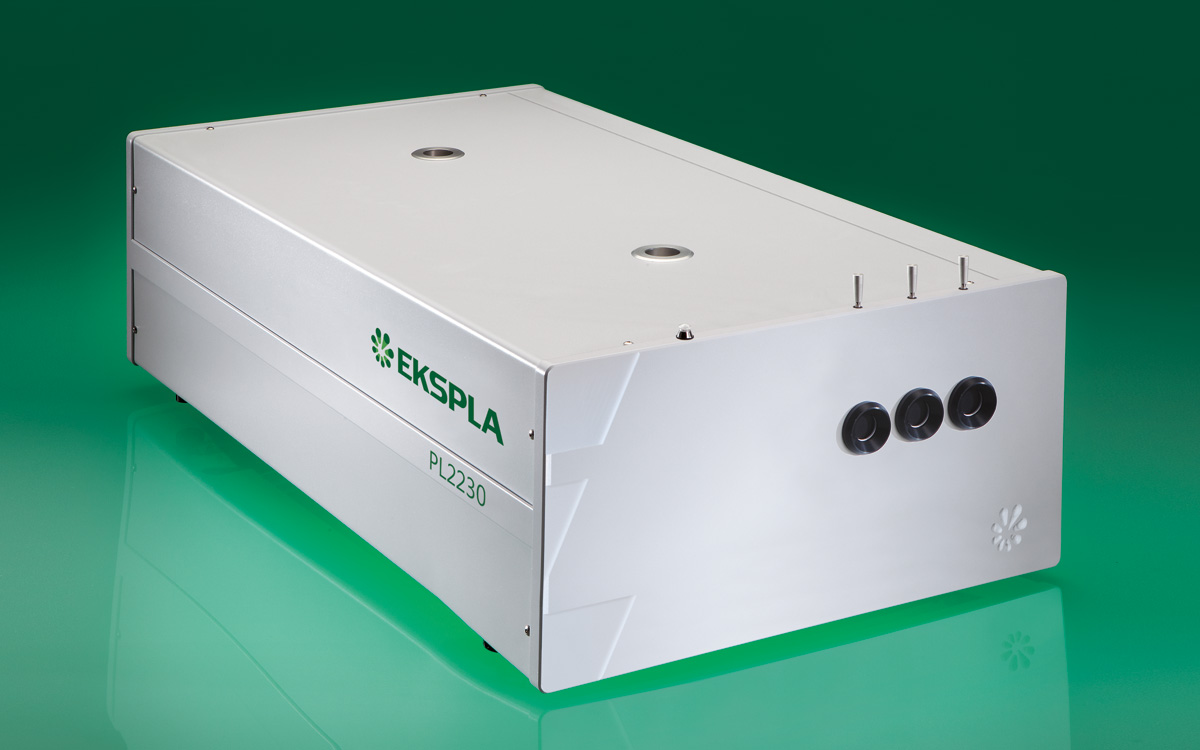
\includegraphics[width=\textwidth]{laser}
	\caption{Pikosekundový laser Ekspla \instrname{PL2231-50}.
		Převzato z~\citeurl{ekspla-datasheet}.}
	\label{fig:instruments-laser}
\end{figure}

\section{ICCD kamera \instrname{Pimax}}
\label{sec:instruments-iccd}

\begin{figure}[htp]
	\centering
	\input{img/cameraeff}
	\caption{Kvantová účinnost kamery deklarovaná výrobcem.}
	\label{fig:instruments-cameraeff}
\end{figure}
